\documentclass[a4paper,12pt]{report}
\usepackage{graphicx}
\usepackage{amssymb}
\usepackage{amsthm}
\usepackage{amsmath}
\usepackage{mathrsfs}
\newtheorem{theorem}{Theorem}
\newtheorem{definition}{Definition}

\begin{document}

%TITLE PAGE
\begin{titlepage}

	\begingroup
	\centering
	{\huge\bfseries Elliptic Curve Cryptography\par}
	\vspace{1cm}
	{\scshape\Large Dissertation\par}
	\vspace{1.5cm}
	{\scshape\LARGE Integrated Masters of Science \par}
	In\\
	{\scshape\LARGE Applied Mathematics \par}
	\vspace{2cm}
	Submitted by\\
	{\Large\itshape Harsh Kumar Chourasia\par}
	\vspace{0.5cm}
	supervised by\\
	Dr. Ram Krishna Panday
	\vspace{0.5cm}

	
\includegraphics[scale=0.75]{logo}

	\vspace{1cm}

	{\scshape\large Department of Mathematics\par}
	{\scshape\large Indian Institute of Technology, Roorkee\par}
	{\scshape\large Department of Mathematics\par}
	{\scshape\large Roorkee-247667\par}
	\endgroup
\end{titlepage}




%DECLARATION PAGE
\pagenumbering{roman}
\section*{Declaration}
\addcontentsline{toc}{section}{\numberline{}Declaration}
I hereby certify that the work which is being presented in the thesis entitled \textbf{Elliptic Curve Cryptography} in the partial fulfillment of the requirement
for the award of the degree of Integrated Master of Science in Applied Mathematics
and submitted to the Department of Mathematics, Indian Institute of Technology
Roorkee, is an authentic record of my own work carried out during a period from
January 2022 to April 2022 under the supervision of \textbf{Dr. R.K. Panday}, Associate Professor, Mathematics Department, Indian Institute of Technology Roorkee.
The matter presented in this report has not been submitted by me for the
award of any other degree of this or any other institute.\\\\\\

\begin{tabular}{l}
	Harsh Kumar Chourasia        \\
	I. M.Sc, Applied Mathematics \\
	Department of Mathematics    \\
	IIT Roorkee                  \\
	Date:                        \\
	Place:                       \\
	\bigskip
\end{tabular}
\hrule
\bigskip
\bigskip
\noindent{\large{\textbf{CERTIFICATE}}} \\\\
This is certified that the above statement made by the candidate is correct to the best of my knowledge.\\\\\\
\vspace{1cm}
\begin{tabular}{l}
	Dr. RK Panday             \\
	Associate Professor       \\
	Department of Mathematics \\
	IIT Roorkee               \\
	Date:                     \\
	Place:                    \\
\end{tabular}
\cleardoublepage
%ABSTRACT PAGE
\section*{Abstract}
\addcontentsline{toc}{section}{\numberline{}Abstract}
This text discuss about Cryptography using Elliptic Curves. It has many practical applications in end-to-end encryption, data and password storing, cryptocurrencies. The motive behind this dissertation is to understand in depth how cryptography is applied in modern technologies such as blockchain which is driving force behind financial revolution of $21^{st}$ century. This dissertation is divided into two chapters. The first chapter deals with the pre-requisite from abstract algebra and number theory that is required to study elliptic curve cryptography. The second chaptes deals with the introduction and algorithms of elliptic curve cryptography.
\cleardoublepage
%ACKNNOWEDGMENTS PAGE	
\section*{Acknowledgments}
\addcontentsline{toc}{section}{\numberline{}Acknowledgments}
I would like to thank my supervisor, Ram Krishna Panday, Department
of Mathematics, Indian Institute of Technology Roorkee for his guidance through each stage of the process.

I would finally like to thank Prof Premananda Bera, Head of Department, Department of Mathematics, Indian Institute of Technology for giving me the permission to carry out this work at IIT Roorkee\\\\\\
\begin{tabular}{l}
	Harsh Kumar Chourasia        \\
	I. M.Sc, Applied Mathematics \\
	Department of Mathematics    \\
	IIT Roorkee                  \\
	Date:                        \\
	Place:                       \\
\end{tabular}

\cleardoublepage


\tableofcontents
\thispagestyle{empty}
\cleardoublepage
\
\setcounter{page}{1}
\pagenumbering{arabic}

\chapter{Pre-requisite}
\large{
This chapter covers topics of Abstract Algebra and Number Theory that are required for cryptography and elliptic curves.}\\
This definition of Group, Ring, Field are as follows
\section{Group}
\begin{definition}
	The set  $G$ is equipped with  single operation $*$ such the the $4$ below properties are satisfied is called a Group.\\
	$(1)$ Closure: $\forall x,y \in G, x*y \in G$ \\
	$(2)$ Additive identity: $\exists 0 \in G$, such that $ \forall x \in G$, $ 0*x=x*0=x$\\
	$(3)$ Associative Property: $ \forall x,y,z \in G$, $(x*y)*z=x*(y*z)$ \\
	$(4)$ Inverse: $ \forall x \in S, \exists y \in G$ such that$x*y=0$ where $y$ is known as inverse of $x$ and is denoted by $x^{-1}$
\end{definition}
\subsection{Abelian Group}
\begin{definition}
	The set $G$ is equipped with  single operation $*$ such the the $5$ below properties are satisfied is called a Abelian Group.\\
	$(1)$ Closure: $\forall x,y \in G, x*y \in G$ \\
	$(2)$ Additive identity: $\exists 0 \in G$, such that $ \forall x \in G$, $ 0*x=x*0=x$\\
	$(3)$ Associative Property: $ \forall x,y,z \in G$, $(x*y)*z=x*(y*z)$ \\
	$(4)$ Commutative Property: $ \forall x,y \in G$, $x*y=y*x$ \\
	$(5)$ Inverse: $ \forall x \in G, \exists y \in G$ such that $x*y=0$ where $y$ is known as inverse of $x$ and is denoted by $x^{-1}$
\end{definition}
So, a abelian group G is a group with $\forall x,y \in G, x*y=y*x$

\section{Ring}
\begin{definition}
	A ring is a set $R$ with two operations $+$ and $*$ which satisfy the below properties\\
	$(1)$ It is abelian group under $+$ \\
	$(2)$ Closure under $*$:  $x,y \in R \Rightarrow	x*y \in R $  \\
	$(3)$ Associative under $*$: $x,y,z \in R \Rightarrow	(x*y)*z=x*(y*z) $\\
	$(4)$ Distributive property $x,y,z \in R$
	$$x*(y+z)=x*y+x*z$$ $$(x+y)*z=x*z+y*z$$
\end{definition}
\section{Field}
\begin{definition}
	A Field is a set $F$ with two operations $+$ and $*$ with following properties \\
	$(1)$Commutative group under $+$\\
	$(2)$Commutative group under $*$\\
	$(3)$Distributive property $x,y,z \in F$
	$$x*(y+z)=x*y+x*z$$ $$(x+y)*z=x*z+y*z$$
\end{definition}
\section{Fermat’s little theorem}
\begin{theorem}
	Let p be any prime number. For any number a such that $p\nmid a$. Then
	$a^{p-1}\equiv 1\pmod p$\\
\end{theorem}
Proof: Assume p is a prime number and $p \nmid a$ \\
Every integer is congruent to one of $0,1,2,\cdots,p-1\pmod p$\\
Only focus on non zero congruence classes, because $0 \pmod p$ contains all the multiples of p (and $p \nmid a$).
Focus on $0,1,2,\cdots,p-1$\\
Multiply all of these by a:
$$a,2a,\cdots,(p-1)a$$
Show that this is a rearrangement of $0,1,2,\cdots,p-1$\\
Case 1: None of these are congruent to 0.\\
Suppose $r.a\equiv 0 \pmod p$\\
Then $p\nmid r.a$, but this is impossible since $p\nmid a$ and $r<p$\\
Case 2: These are distinct, no two are congruent to each other.\\
Pick two values $r.a$,$s.a$\\
$$0<r<p$$
$$0<s<p$$
Let's show that $r.a \not\equiv s.a \pmod p$\\
So look at $r.a-s.a=(r-s).a$. As $p\nmid a$, so can $p \mid (r-s)?$\\
$$0<r<p$$
$$-p<-s<0$$
Adding these inequalities gives you:
$$-p<r-s<p$$
So, $p\nmid(r-s)$ which means $a,2a,\cdots,(p-1)a$ is a rearrangement of\\ $1,2,\cdots,(p-1).$
$$a,2a,\cdots,(p-1)a\equiv 1,2,\cdots,(p-1) \pmod p$$
$$(p-1)!a^{p-1}\equiv (p-1)! \pmod p$$
$$a^{p-1}\equiv 1 \pmod p$$



\cleardoublepage

\chapter{Elliptic Curves and Cryptography}
\section{Introduction to Cryptography}
The written word is the most important invention in human history. But as long as human has the ability to share information, they have also had the need to conceal that information as well. This need lead to invention of cryptography.\\
The word cryptography comes from greek which means "hidden writing". According to Wikipedia, \textbf{Cryptography, or cryptology is the practice and study of techniques for secure communication in the presence of adversarial behavior.}
\\Some of the application of Cryptography includes:
\begin{itemize}
	\item End-to-end Encryption for e-mail, messaging apps, GSM phones.
	\item Storing Data: Biggest consumer application of cryptography includes Kindle, iPod which stores books and songs in encrypted format to protect copyright.
	\item Storing Password: Storing passwords in plane text is not secure. If an attacker has access to the system they can read the password. If the password is converted into hash using one way mapping function and stored. Every time a user logs in, the password will be converted into hash and compared with the stored password.
\end{itemize}
There are mainly two type of cryptography: Symmetric key cryptography and Asymmetric key cryptography.


\subsection{Symmetric cryptography}
Let Alice want to share a message m with Bob. They do so by using a common key and knowledge of some algorithm to encrypt and decrypt message. Alice encrypts the message using the key to produce the cipher text. Now Bob can use key with cipher text to decrypt message.

In symmetric cryptography a common key is used by the sender and receiver.
\vspace{2cm}

\begin{figure}[h!]
	\begin{center}
		\caption{A picture of the universe!}
		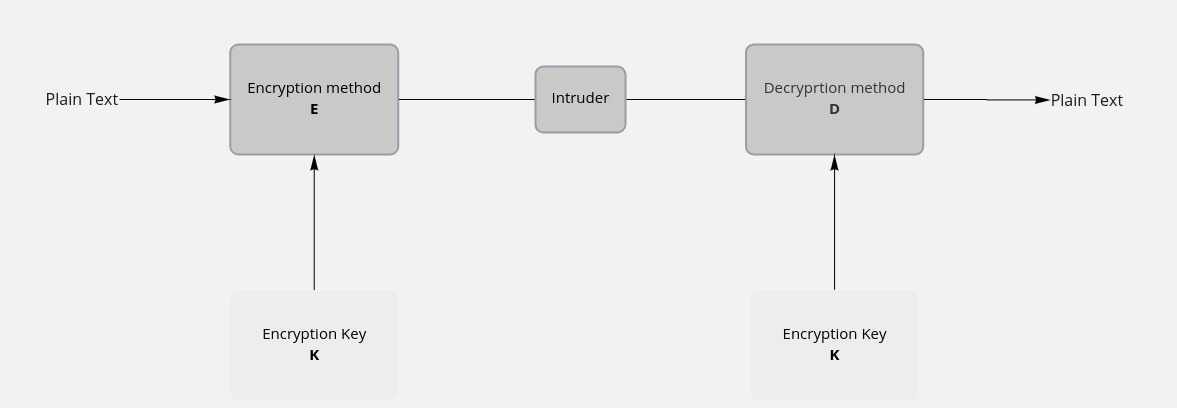
\includegraphics[scale=0.36]{sym}
	\end{center}
\end{figure}

\vspace{2cm}
\subsection{Asymmetric cryptography}
Asymmetric cryptography works by using private and public key pairs.
Each user has a private,public key pair. Public key can be shared freely across the network and is used to verify the owner of a message.
Private keys is not transmitted across the network. Public are used to encrypt the message and private key is used to decrypt the message. The major advantage of asymmetric cryptography is that there is no need of a shared key. \\

\begin{figure}[h!]
	\begin{center}
		\caption{A message exchange using private and public keys}
		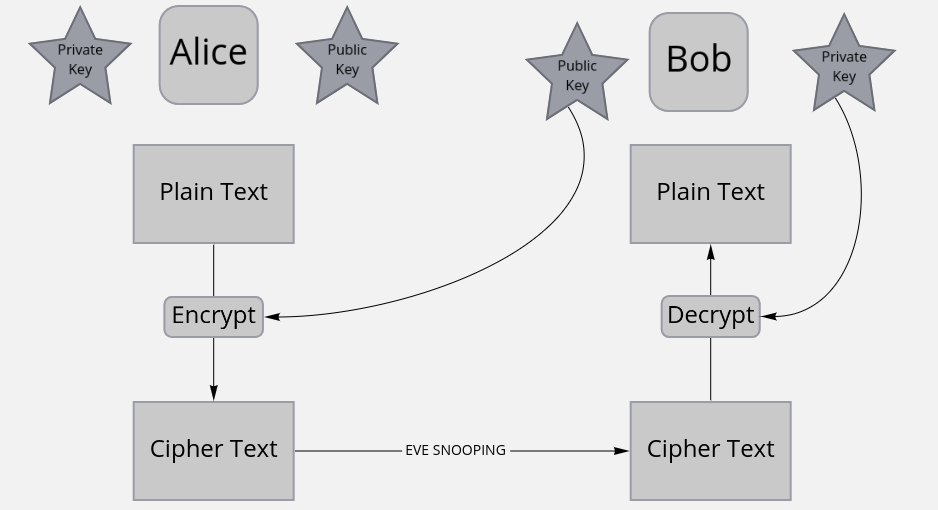
\includegraphics[scale=0.36]{asym}
	\end{center}
\end{figure}


\section{Elliptic Curves}
Equation of type $ y^2 = x^3+ax+b $ are called Weierstrass equations. It is named after Karl Weierstrass $(1815-1897)$ who studied them in $19^{th}$ century. \\
\begin{definition}
	Elliptic curves are solution sets of Weierstrass equations
	$$E:y^2 = x^3+ax+b ...(1)$$ with  $ \{\ \mathscr{O}  $ \}\ where $\Delta_E = 4a^3+27b^2\neq 0$.
	$\Delta_E \neq 0$ guarantees that the equation $x^3+ax+b$ has no repeated roots i.e.
	$ x^3+ax+b=(x-e_1)(x-e_2)(x-e_3)$ where $e_1,e_2,e_3$ are distinct. $  \mathscr{O}  $  is defined as the point at infinity which lies on every vertical line.\\
\end{definition}

\begin{figure}[h!]
	\caption{Example of Elliptic Curves}
	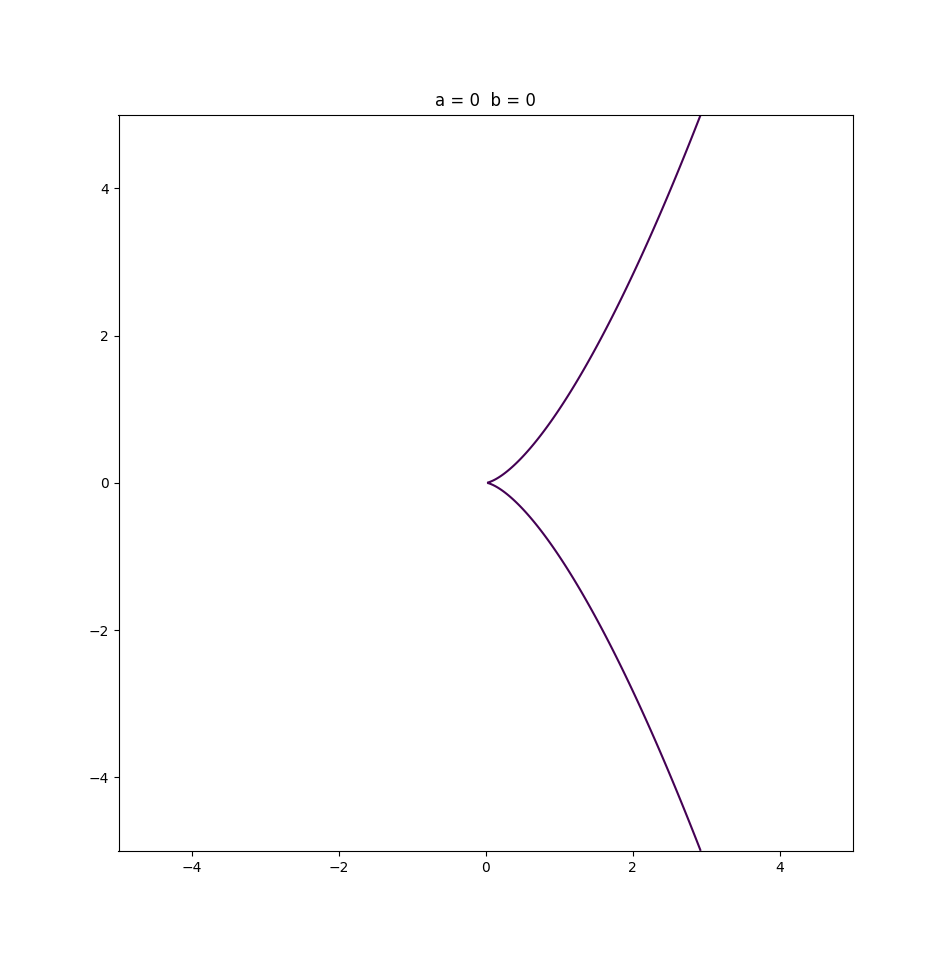
\includegraphics[scale=0.30]{Figure_1}
	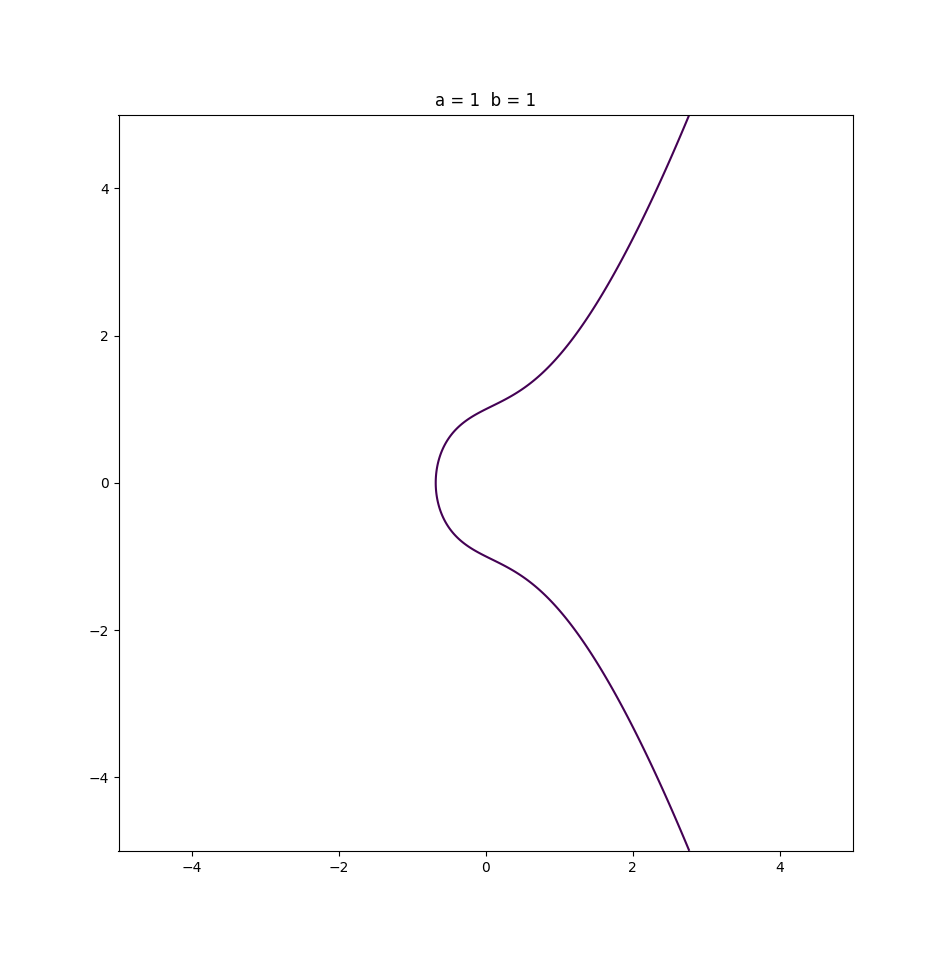
\includegraphics[scale=0.30]{Figure_2}\\
	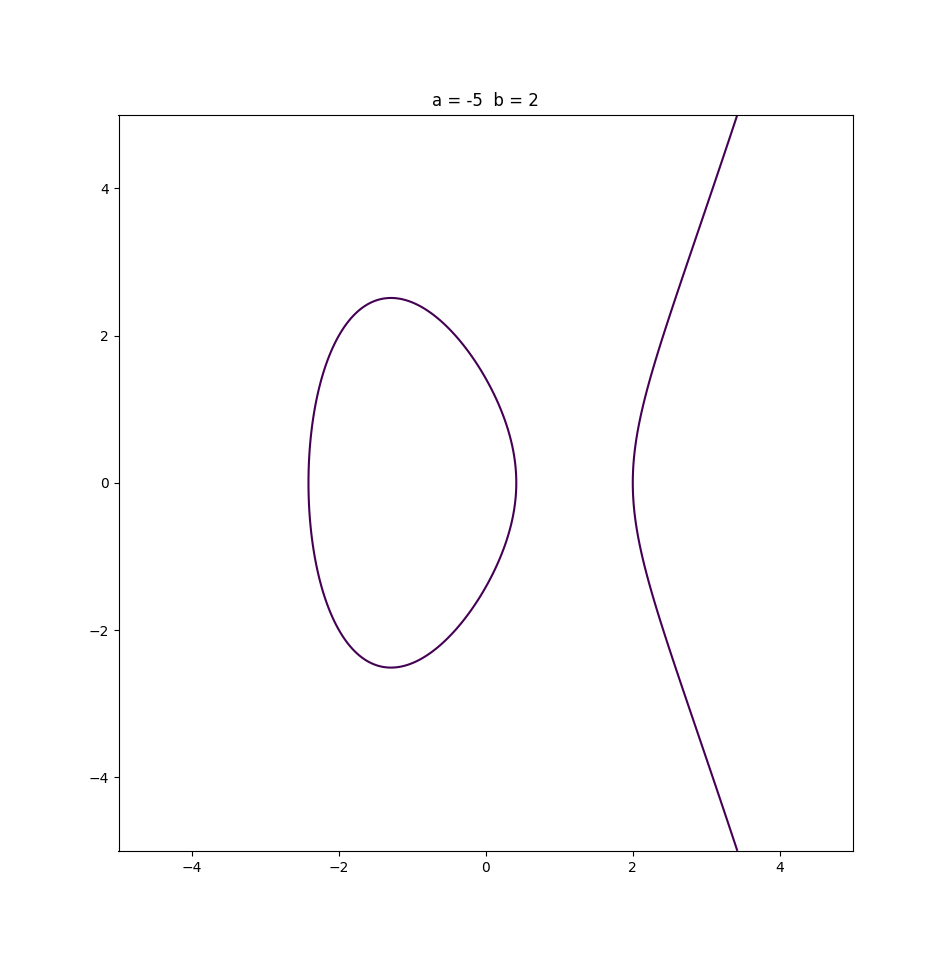
\includegraphics[scale=0.30]{Figure_3}
	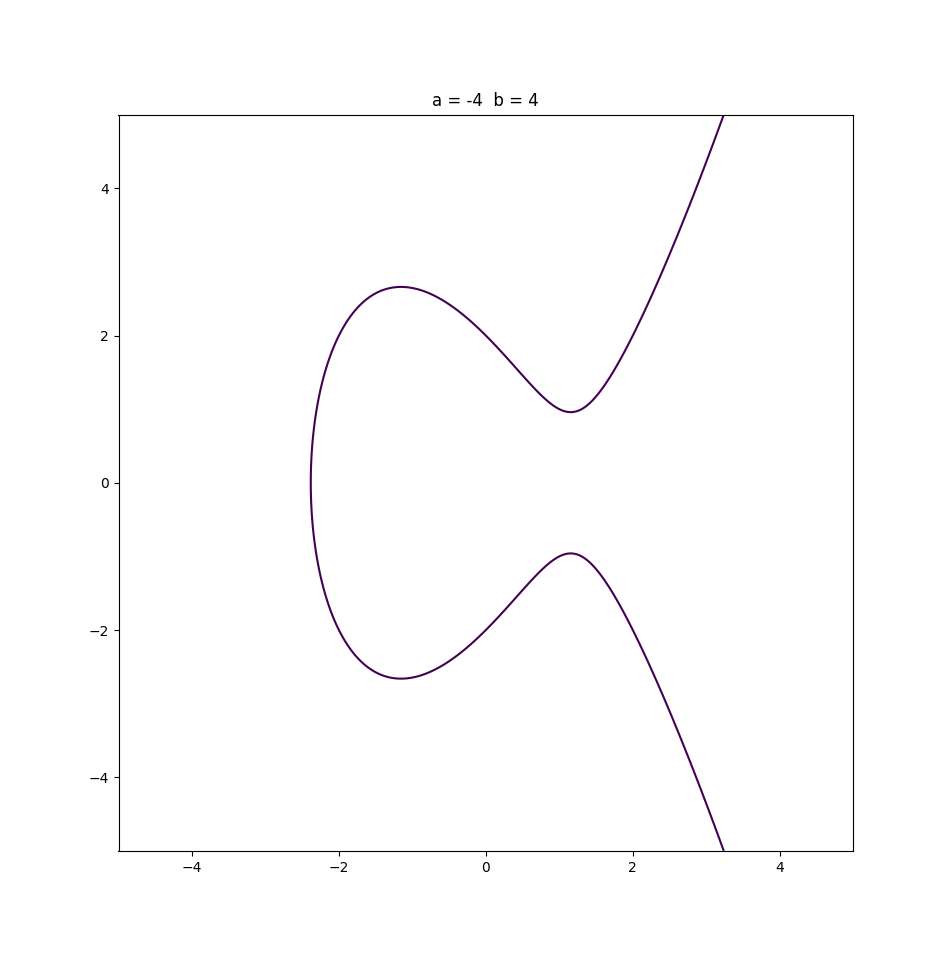
\includegraphics[scale=0.30]{Figure_4}
\end{figure}
\cleardoublepage
If (x,y) satisfies eq(1), then (x,-y) is also a solution of equation (1). So, elliptic curves are symmetric about x-axis. \\
The definition of addition "$+$" operator is a not the usual definition one might expect
$$(a,b)+(c,d) \neq (a+c,b+d)$$
Two points $P_1$ and $P_2$ on elliptic curve. If we make a line L that passes through $P_1$ and $P_2$, it will intersect the curve at point $P_3=(x_3,y_3)$. The reflection of $P_3$ from x-axis i.e. $(x_3,-y_3)$ is called the sum of points $P_1$ and $P_2$
\begin{figure}[h!]
	\begin{center}
		\caption{Example of $P_1+P_2$}
		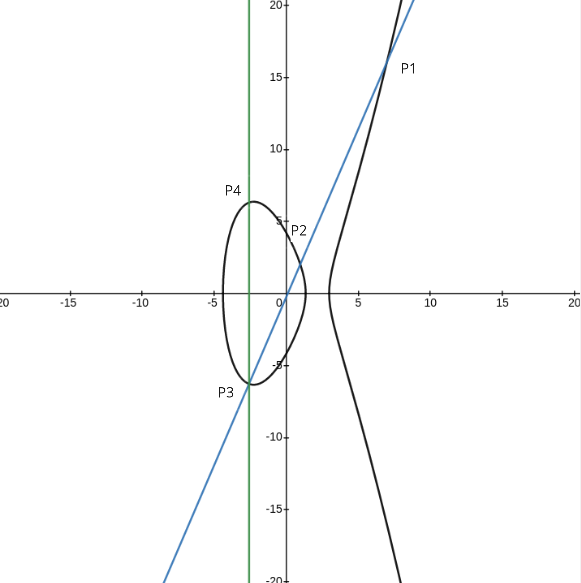
\includegraphics[scale=0.4]{2}
	\end{center}
\end{figure}
So, what is $P_1+P_1$? This is the limiting case where $P_2 \to P_1$ and the Line L becomes the tangent to E at $P_1$. This line will intersect E at $P_3$. The reflection of $P_3$ about x-axis  is $P_1+P_1$.
\begin{figure}[h!]
	\caption{Example of $P_1+P_1$}
	\begin{center}
		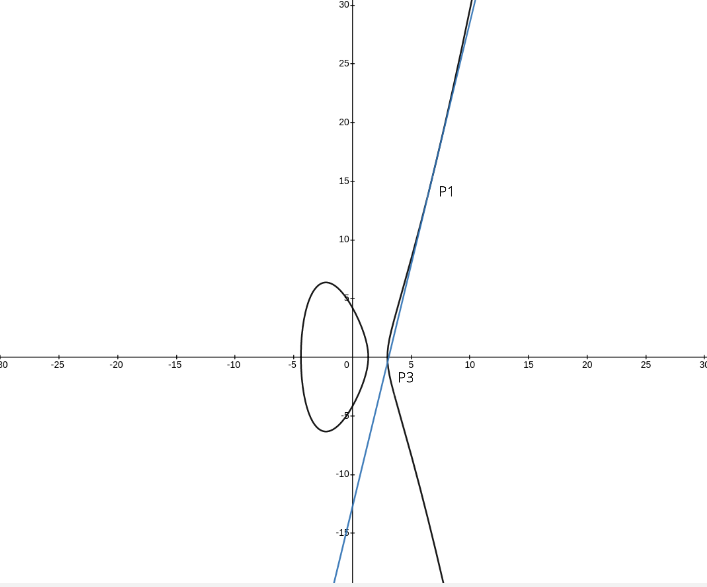
\includegraphics[scale=0.3]{3}
	\end{center}
\end{figure}
Let's look at the case when two points on the curve when $P_1=(x,y)$ and $P_2=(x,-y)$ are added. In this case line L is $x=a$. L will not intersect the curve at third point. In this case we define
$ P_1+P_2= \mathscr{O} $. We define $\mathscr{O}$  as the point in infinity that lies on every vertical line.
If P = (x,y) then -P is defined as (x,-y). So, $P+(-P)=\mathscr{O}$...(2)
\begin{figure}[h!]
	\begin{center}
		\caption{Example of $P_1+(-P_1)=\mathscr{O}$}
		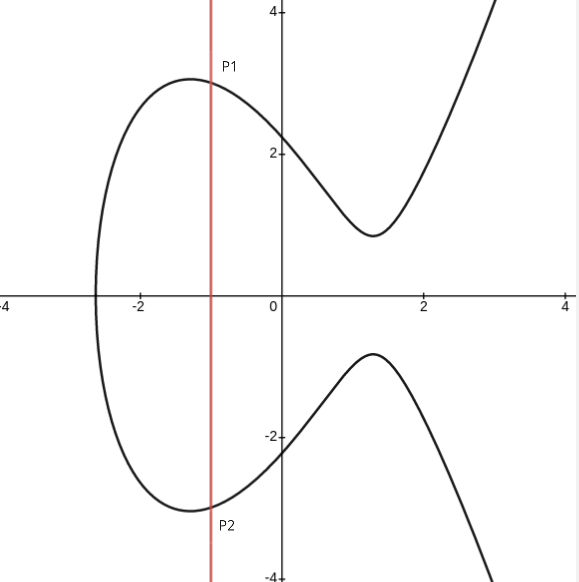
\includegraphics[scale=0.3]{1}
	\end{center}
\end{figure}
\cleardoublepage
\begin{theorem}
	Let $P=(x_1,y_1)$ and $Q=(x_2,y_2)$ be two points on elliptic curve $E:Y^2=X^3+
		AX+B$. Then the following are true:
	\begin{enumerate}
		\item If $P=\mathscr{O}$, then $P+Q=Q$
		\item If $Q=\mathscr{O}$, then $P+Q=P$
		\item If $P=-Q$ then $P+Q=\mathscr{O}$
		\item If $P \neq Q$ then $\lambda = (y_2-y_1)/(x_2-x_1)$ and if $P=Q$ then\\ $\lambda = (3x_1^2+A)/(2y_1)$. In both cases,
		      \\$P_1+P_2 = (\lambda ^2 - x_1 - x_2, \lambda (x_1 - x_3)-y_1)$
	\end{enumerate}
\end{theorem}
\begin{proof}
	$(1),(2),(3)$ are true as discussed above.\\
	(4) If $P\neq Q$ then $\lambda$ is the slope of the line passing through $P$ and $Q$. If $P=Q$ then $\lambda$ is the slope of the tangent at $P$. Suppose Line $y=\lambda x+c$ intersects the curve at $(x_3,y_3)$ in addition to $(x_1,y_1)$ and $(x_2,y_2)$.
	$$(\lambda x+c)^2=x^3+Ax+B$$
	$$x^3-\lambda ^2 x^2 +(A-2c\lambda)x+(B-c^2)=(x-x_1)(x-x_2)(x-x_3)$$
	We get $x_3 = \lambda ^2-x_1-x_3$ by comparing the coefficients of $x^2$. $y_3=\lambda x+c=y_1-\lambda(x_1-x_2)$. The ordinate of $P+Q$ is $-y_3=\lambda (x_1 - x_3)-y_1)$
\end{proof}
\begin{theorem}
	Let E be Elliptic curve. Then $E$ forms abelian group under addition. The following statements are true:
	\begin{enumerate}
		\item $P_1+\mathscr{O}=\mathscr{O}+P_1=P_1$ for all $P_1 \in E$
		\item $P_1+(-P_1)=\mathscr{O}$ for all $P_1 \in E$
		\item $(P_1+P_2)+P_3=P_1+(P_2+P_3)$ for all $P_1,P_2,P_3 \in E$
		\item $P_1+P_2=P_2+P_1$ for all $P_1,P_2 \in E$
	\end{enumerate}
\end{theorem}
\begin{proof}
	(1) Claim: $P_1+\mathscr{O}=P_1$ \\
	If a line is drawn through P and $\mathscr{O}$ it will intersect E at -P. Reflection of -P from x-axis is again P. So, $P_1+\mathscr{O}=P_1$
	Similarly, $\mathscr{O}+P_1=P_1$\\
	(2) Explained above in equation (2)\\
	(3) Associative property is non-trivial to prove using geometry. It can be verified by using Theorem 2 by calculation using substitution.\\
	(4) is true as line passing through $P_1$ and $P_2$ is same as the line passing through $P_2$ and $P_1$.
\end{proof}
\cleardoublepage
\section{Elliptic curves over finite fields}
\begin{definition}
	Elliptic curve over a finite field $F_p$ is defined as equation of the form $$E:y^2 = x^3+ax+b$$ where $a,b\in F_p$ and $\Delta_E = 4a^3+27b^2\neq 0$.
\end{definition}
Example:
Let's suppose $a=0$, $b=1$ and $p=11$. \\
$F_{11}=\{0,1,2,3,4,5,6,7,8,9,10\}$.$\{a,b\}\in F_{11}$ and $4*0^2+27*1^3=27\neq 0$. Hence, $E:y^2 = x^3+1 \pmod {11} $ is an elliptic curve over finite field. \\
$E(F_{11}) = \{\mathscr{O},(10,0),(0,10),(0,1),(9,2),(9,9),(2,3),(2,8),(6,8),$\\$(8,4),(8,7),(3,5),(3,6)\}$
with $|E(F_{11})|=12$
\begin{theorem}
	Equation of elliptic curve over finite field $F_p$ is $E : Y^2=X^3+
		AX+B$. Let $P=(x_1,y_1)$ and $Q=(x_2,y_2)$ be two points on $E$. If Theorem 2 is applied to points $P$ and $Q$ then the resulting point also lies on $E$.
\end{theorem}
\begin{proof}
	Theorem 2 is derived by substituting the equation of line to elliptic curve. So the solution automatically satisfies the elliptic curve. Similarly Theorem 4 is also true.\\
\end{proof}
Example: Consider the above example. Let $P=(0,1)$ and $Q=(10,0)$.
$\lambda = \frac{1-0}{0-10} = \frac{1}{-	10} = 1 \pmod{11}$,$x_3=1-0-10=-9=2 \pmod{11}$\\ $y_3=1(0-(2))-1=-3=8$ and $(2,8) \in E$ \begin{theorem}
	The elliptic curve over finite field along with addition property forms finite group.
\end{theorem}

\cleardoublepage
\section{Elliptic curve discrete logarithm problem}

\begin{definition}
	Let $(G,.)$ be a group and $g$ be the generator of the group and $h\in G$ such that $$g^x=h$$
	$x$ is called discrete logarithm of $h$ base $x$ and is denoted by $x=log_g h$.
\end{definition}
Elliptic curve group operation is addition as described above.So, in case of elliptic curve discrete logarithm problem is described as follows:
Let $P,Q \in E$ such that $nP=Q$. $n$ is called elliptic discrete logarithm of $Q$ base $P$ and is denoted by $n =\log_P Q$.

It should be noted that if $Q$ is not multiple of $P$ then $n$ will not be defined. But for all practical purposes $Q$ is obtained from repeatedly adding $P$. So $n$ will exist.

We also note that in every finite group every element has finite order. Let order of $P$ be $s$ i.e. $s P=\mathscr{O}$. If $n_0$ is the smallest number satisfying $Q=sP$. Then for all $n=n_0+is$ $ \forall i \in \mathbb{Z} $, $Q=nP$.It implies $\log_P Q$ is an element of  $\mathbb{Z}/s\mathbb{Z}$.We could also set the value to be $n_0$.But if we define the value to be in $\mathbb{Z}/s\mathbb{Z}$ the the following equation is satisfied.
$$\log_P(Q+R)=\log_P(Q)+\log_P(R)$$
Therefore the function
$log_P:E(F_p)\rightarrow \mathbb{Z}/s\mathbb{Z}$ defines group homomorphism.
\subsection{Double and Add Algorithm}
The value of $n$ in $Q=nP$ is large for practical application.If $nP$ is calculated by adding $P$ repeatedly $n$ number of times, it will $O(n)$ operation. Suppose $n$ has $k$ binary digits. Then the complexity will be $O(2^k)$. By the use of double and add algorithm we can reduce the complexity to $O(\log {n})$ or $O(k)$.\\
Take $n=151$. Binary representation of 151 is $10010111_2$.
$$151=1.2^7+0.2^6+0.2^5+1.2^5+0.2^4+1.2^3+1.2^2+1.2^1+1.2^0$$
$$or$$
$$151P = 2^7P+2^4P+2^2P+2^1P+2^0P$$
Obtain $151P$ using double and add algorithm
\begin{enumerate}
	\item Start with $P$
	\item Double it to get $2P$ ($P+P$)
	\item Add $2P$ to $P$ (result will be $2^1P+2^0P$)
	\item Double $2P$ to get $4P$ ($2P+2P$)
	\item Add $4P$ to the result (result will be $2^2P+2^1P+2^0P$)
	\item Double $4P$ to get $8P$ ($4P+4P$)
	\item Double $8P$ to get $16P$ ($8P+8P$)
	\item Add $16P$ to the result (result will be $2^4P+2^2P+2^1P+2^0P$)
	\item Keep Doubling $16P$ till $128P$ is obtained
	\item Add $128P$ to the result (result will be $2^7P+2^4P+2^2P+2^1P+2^0P$)
\end{enumerate}
We obtained $151P$ using only four addition and seven doubling operation!
\cleardoublepage
\textbf{Pseudo-code of double and add algorithm}\\
Let $n=n_0+2n_1+2^2n_2+...+2^mn_m$ where $n_0,...n_m \in {0,1}$,$m =\lfloor \log_2 {n} \rfloor$
\begin{enumerate}
	\item $bits = [n_0,n_1,...n_m]$
	\item $result=\mathscr{O}$ \hspace{10mm} //  infinity point
	\item $temp=P$
	\item for bit in bits:
	\item \hspace{10mm}  if bit == 1:
	\item \hspace{10mm} \hspace{10mm}  result = result + temp \hspace{10mm} // addition operation
	\item \hspace{10mm} temp = temp + temp \hspace{10mm}  // doubling operation
	\item return result
\end{enumerate}
\subsection{Hasse's Theorem}
Hasse's Theorem is used to estimate number of points in an elliptic curve over finite field. We state Hasse's theorem without proof.
\begin{theorem}
Let $N$ be the number of points on an Elliptic Curve $E$ over finite field $F_q$. Then the following inequality is true
$$|N-(q+1)|<2\sqrt{q}$$ 
$$or$$
$$q+1-2\sqrt{q}<N<q+1+2\sqrt{q}$$
\end{theorem}

\subsection{How to solve ECDLP}
Suppose  $P$ and $Q$ are points on an Elliptic Curve $E$ over finite field $F_p$ such the $Q=nP$. The value of $P$ and $Q$ are known and we wish to find the value of $n$.\\\\
\textbf{Exhaustive Search Method}\\
Compute the value of $P,2P,3P...$ until you find a multiple such that it is equal to $Q$. Time complexity of this algorithm is $O(p)$.\\\\
\textbf{Collision Search Method}\\
Compute two lists for randomly chosen integers $m_1, m_2, . . .m_r$ and $n_1, n_2, . . .n_r$ where each integer is between $1$ and $p$.\\
List 1: $m_1 P, m_2 P, . . .,m_r P$\\
List 2: $n_1 P + Q, n_2 P + Q, . . ., n_r P + Q$\\
As soon as we find $m_u P$ and $m_v P + Q$ such that $m_u P = m_v P + Q$, then $Q = (m_v - m_u) P $ i.e. $n=m_v - m_u$. Time complexity of this algorithm is $O(\sqrt{p})$ by the birthday paradox.\\\\\\
The value of $p$ is taken very large for practical purpose. For example, Secp256k1 is the name of the elliptic curve used by Bitcoin to implement its public key cryptography. The value of $p$ used by it is $p = 2^{256} – 2^{32} – 2^9 – 2^8 – 2^7 – 2^6 – 2^4 – 1$
\section{Elliptic Diffie–Hellman key exchange}
In this section we will use Elliptic curve to do cryptography. The biggest problem of symmetric cryptography is sharing of private keys. Historically secret key used to be shared physically and then the encrypted message were shared over public channel. Diffie-Hellman key exchange helps sender and receiver of the message to securely exchange cryptographic keys over public channel. It's security does depend on mathematical principle. \\\\
Elliptic Diffie–Hellman Key Exchange Algorithm
\begin{enumerate}
	\item A large prime number $p$, an Elliptic Curve $E$ over $F_p$ and a point $P \in E(F_p)$  is shared between Ram and Shayam over public channel.
	\item Ram chooses a large random number $n_R$ and computes $Q_R = n_R P$
	\item Shayam chooses a large random number $n_S$ and computes $Q_S = n_S P$
	\item Ram and Shayam shares $Q_R$ and $Q_S$ over the public channel.
	\item Ram now compute $n_R Q_S$
	\item Shayam now compute $n_S Q_R$
	\item The shared secret key is $Q=n_R Q_S=n_R (n_S P)=n_S (n_R P)=n_S Q_R$
\end{enumerate}
Suppose Ghanshyam wants to obtain the secret key. Ghanshyam knows the value of $P$, $Q_R$, $Q_S$ as they are available on public channel. Ghanshyam can solve Elliptic Curve Discrete Logarithm Problem i.e. the equation $Q_R = n_R P$ or $Q_S = n_S P$ to obtain the value of $n_R$ and $n_S$ respectivly. After the the value of $Q$ can be obtained using the formula $Q=n_R Q_S$ or $Q=n_S Q_R$. 
\bibliographystyle{plain}
\bibliography{bibliography}
\end{document}
